% Restructured book: evaluation of automatic layout design.
\chapter{Evaluation of Automatic Interior Layout Design}
\label{chap:layout-evaluation}

This chapter evaluates the \textbf{Automatic Interior Layout Design} component presented in Chapter~4. The evaluation focuses on whether RoomFlow can generate editable furniture layouts that are geometrically valid, aligned with the design brief, functionally usable, and stable across repeated runs. The chapter is organized around two experiments. Experiment~1 compares the complete RoomFlow pipeline with two external baselines, I-Design and FlairGPT, under the same benchmark cases and scoring protocol. Experiment~2 performs an ablation study to examine whether the main components of RoomFlow, including semantic planning, geometric solving, and final layout selection, contribute measurable improvements to the final layout quality.

The layout benchmark is executed as a controlled offline evaluation. Each benchmark case contains a room type, a boundary polygon, optional doors and windows, and a natural-language design brief. One \emph{case-run observation} is one system output for one benchmark case in one repeated run. Ideally, each case should be executed five times to better capture the non-deterministic behavior of AI-assisted generation. However, because repeated execution requires substantial model-calling cost and manual/evaluator processing time, each benchmark case is executed twice in this thesis. The scores are then aggregated by benchmark group and opening condition, allowing the evaluation to separate case diversity from repeated-run variation.

\section{Benchmark Dataset}\label{subsec:eval-layout-benchmark-cases}

The benchmark for \textbf{Automatic Interior Layout Design} uses controlled cases created for this thesis, inspired by real-world layouts rather than copied directly. This choice allows the evaluation to vary one difficulty factor at a time, such as room shape, opening placement, or object requirements, while keeping the scoring protocol comparable across systems. The cases are still realism-oriented: they use common bedroom and living-room dimensions, typical furniture groups, and fixed doors or windows that create practical placement constraints.

The benchmark contains 50 cases. Twenty cases are minimal rectangular rooms defined only by their length and width, split equally between rooms without openings and rooms with a door and window. Another twenty cases are detailed rectangular rooms with explicit furniture and functional requirements, again split equally by opening condition. The remaining ten cases use non-rectangular boundaries; two omit openings and eight combine irregular geometry with doors or windows. Each case stores the room type, polygon vertices in millimeters, opening segments, room metadata, and natural-language design brief.

Each case also includes an expected-output specification used for evaluation. This specification records required object categories, allowed count ranges, a minimum usable-object count, and any case-specific spatial relations that should be checked. It does not define a single target layout, because several different arrangements may satisfy the same room brief. For this reason, the generated output is evaluated by constraint satisfaction and layout quality rather than by exact similarity to one hand-authored reference layout.

Before scoring, every system output is normalized into a common object schema containing object category, footprint, position, and orientation. The evaluator then checks whether the layout stays inside the room, avoids invalid overlaps, keeps openings usable, follows the requested objects and relations, provides a usable arrangement, and includes enough valid objects. Experiment~2 additionally uses a 10-case robustness holdout with richer style, material, palette, and gallery-diversity targets. The three benchmark groups used by the layout experiments are summarized in Table~\ref{tab:7-3}.

\begingroup
\small
\setlength{\tabcolsep}{4pt}
\renewcommand{\arraystretch}{1.15}
\begin{xltabular}{\textwidth}{|>{\raggedright\arraybackslash}p{0.24\textwidth}|>{\raggedright\arraybackslash}p{0.20\textwidth}|>{\raggedright\arraybackslash}p{0.44\textwidth}|}
\caption{Benchmark groups for Automatic Interior Layout Design.}\label{tab:7-3}\\
\hline
\textbf{Benchmark group} & \textbf{Purpose} & \textbf{Main characteristics} \\
\hline
Simple sanity scenarios & Explain the pipeline and metrics with easy cases & Minimal room description, rectangular shape, with or without openings \\
\hline
Regular rectangular scenarios & Evaluate common living-room and bedroom situations & Rectangular room, detailed prompt, required objects, optional doors/windows \\
\hline
Non-rectangular challenging scenarios & Evaluate solver and constraint handling under difficult geometry & L-shaped, chamfered, side-recess, or bay-like room, detailed prompt, mixed openings \\
\hline
\end{xltabular}
\endgroup

A typical example is a compact bedroom measuring approximately \(4.0m \times 3.2m\), featuring a door on the south wall and a window on the north wall. The design brief requires placing a bed, wardrobe, bedside table, and a small work desk while maintaining sufficient walking space. Even in this straightforward scenario, the system must ensure proper containment, keep openings unobstructed, include all required objects, and maintain functional circulation.

\section{Evaluation Metrics}\label{subsec:eval-layout-metrics}

Before scoring the full benchmark, each system output is normalized into the same 2D layout schema. This normalization makes the comparison independent of each system's original output format. Each normalized layout contains the room boundary, furniture categories, object footprints, positions, and orientations. The evaluator then measures whether the layout is spatially feasible, follows the design brief, supports functional use, and retains enough usable furniture.

Both experiments use four primary component metrics and one weighted overall score. The four primary metrics are \textbf{Spatial Feasibility}, \textbf{Design Brief Compliance}, \textbf{Functional Arrangement Quality}, and \textbf{Usable Object Completeness}. All scores are reported on a 0--100 scale, where higher is better. Experiment~2 keeps these shared metrics and adds a separate robustness holdout because the primary metrics do not fully measure style-material consistency, gallery diversity, reliability, or lower-tail behavior across repeated runs. Table~\ref{tab:7-4} summarizes the interpretation of each metric group before the detailed formulas are introduced in the following subsections.

\begingroup
\small
\setlength{\tabcolsep}{4pt}
\renewcommand{\arraystretch}{1.15}
\begin{xltabular}{\textwidth}{|>{\raggedright\arraybackslash}X|>{\raggedright\arraybackslash}X|>{\raggedright\arraybackslash}X|}
\caption{Layout metric groups and evaluation interpretation.}\label{tab:7-4}\\
\hline
\textbf{Question} & \textbf{Metric group} & \textbf{Evaluation interpretation} \\
\hline
Is the layout physically possible? & Spatial feasibility & Checks whether furniture footprints stay inside the room, avoid blocking overlaps, keep doors and windows usable, and leave a basic path from the door to the room interior. \\
\hline
Does the layout follow the design brief? & Design brief compliance & Checks whether the requested objects, expected counts, and key spatial relations are present. For example, a sofa should face the TV if the brief asks for a media area. \\
\hline
Is the room comfortable to use? & Functional arrangement quality & Checks whether the valid objects form a sensible room arrangement: main furniture should be reachable, circulation should remain open, and the arrangement should not feel awkward. \\
\hline
Are enough usable objects included? & Usable object completeness & Checks whether enough main blocking furniture remains after invalid out-of-room or overlapping objects are discounted. It is a minimum furnishing sufficiency check, not a direct measure of whether every requested object is valid. \\
\hline
Is the system reliable across runs? & Robustness & Checks whether repeated runs maintain good quality and return useful gallery variants instead of occasionally collapsing into poor or duplicate outputs. \\
\hline
\end{xltabular}
\endgroup

The four primary metrics are designed specifically for this benchmark rather than copied directly from a single standard benchmark. They are informed by common evaluation signals in indoor-layout and text-to-3D scene-generation studies, including out-of-boundary checks, overlap checks, accessibility, object selection, and instruction alignment. The purpose of the metric set is not to claim a universal standard for interior layout evaluation, but to provide a transparent and repeatable scoring protocol for the benchmark used in this thesis.

The following subsections define each metric in more detail. Spatial feasibility focuses on hard spatial constraints. Design brief compliance evaluates whether the generated layout satisfies the user's brief. Functional arrangement quality measures practical usability among the valid objects. Usable object completeness checks whether enough main furniture remains after invalid objects are discounted, so it should be read together with the other metrics rather than as a complete request-following score. The final overall score combines these components with fixed weights, while the additional ablation metrics evaluate robustness-related behavior.

All component scores are reported on a 0--100 scale, using the following clipping function:
\[
\mathrm{clip}_{0,100}(x)=\min(100,\max(0,x)).
\]
Let \(n_{\mathrm{oob}}\), \(n_{\mathrm{overlap}}\), \(n_{\mathrm{open}}\), and \(n_{\mathrm{access}}\) denote the numbers of out-of-room blocking objects, overlapping blocking-object pairs, opening-clearance violations, and blocked door-to-room-center access paths. Let \(A_{\mathrm{oob}}\) and \(A_{\mathrm{overlap}}\) denote the corresponding total violation areas in \(\mathrm{mm}^{2}\).

\subsection{Spatial Feasibility}
This metric captures basic physical feasibility, following the use of out-of-boundary and overlap-related checks in LayoutGPT, I-Design, and FlairGPT~\cite{al2023LayoutgptCompositionalVisual,al2024IDesignPersonalized,Littlefair2025FlairgptRepurposingLlms}.
\[
\begin{aligned}
S_{\mathrm{spatial}}=\mathrm{clip}_{0,100}\bigl(
100
&-22n_{\mathrm{oob}}-24n_{\mathrm{overlap}}
-16n_{\mathrm{open}}-12n_{\mathrm{access}}\\
&-\min(A_{\mathrm{oob}}/40000,18)
-\min(A_{\mathrm{overlap}}/50000,18)
\bigr).
\end{aligned}
\]
The area terms make large boundary or overlap violations worse than small numerical contacts, while the clipping keeps the score within the common 0--100 range.

\subsection{Design Brief Compliance}
This metric checks whether the generated layout satisfies the case-specific design-brief requirements encoded in the benchmark, including required objects, expected object counts, and key spatial relations; it follows the broader instruction-alignment perspective used in LLM-based scene-generation systems~\cite{al2023LayoutgptCompositionalVisual,al2024IDesignPersonalized}.
\[
S_{\mathrm{brief}} =
\begin{cases}
100, & N_{\mathrm{checks}}=0,\\
100 \cdot \dfrac{N_{\mathrm{passed}}}{N_{\mathrm{checks}}}, & N_{\mathrm{checks}}>0.
\end{cases}
\]
Here \(N_{\mathrm{checks}}\) is the number of benchmark checks applicable to the case and \(N_{\mathrm{passed}}\) is the number satisfied by the output.

\subsection{Functional Arrangement Quality}
This metric is a conservative proxy for practical room usability, motivated by layout-coherence, accessibility, and functional-placement criteria discussed in HOLODECK and FlairGPT~\cite{al2024HolodeckLanguageGuided,Littlefair2025FlairgptRepurposingLlms}.
\[
S_{\mathrm{function}}=\mathrm{clip}_{0,100}\bigl(
100
-18n_{\mathrm{overlap}}-14n_{\mathrm{oob}}
-12n_{\mathrm{open}}-10n_{\mathrm{access}}
\bigr).
\]
Unlike spatial feasibility, this score uses only count-based penalties because it is meant to summarize whether repeated spatial incidents make the room hard to use.

\subsection{Usable Object Completeness}
This metric is adapted from object-selection and object-coverage signals in prior work, but applies a stricter lower-bound definition: it counts only main blocking furniture that remains usable after invalid out-of-room or overlapping objects are excluded~\cite{al2024IDesignPersonalized,al2024HolodeckLanguageGuided,Littlefair2025FlairgptRepurposingLlms}. It does not replace design brief compliance; instead, it checks whether the layout still contains enough usable core furniture after geometric filtering.
\[
S_{\mathrm{usable}} =
\begin{cases}
100, & N_{\min}\ \text{is not specified},\\
\mathrm{clip}_{0,100}\bigl(100-18\max(N_{\min}-N_{\mathrm{valid}},0)\bigr), & \text{otherwise}.
\end{cases}
\]
Here \(N_{\min}\) is the minimum expected number of usable blocking objects and \(N_{\mathrm{valid}}\) is the number that remains after excluding invalid objects.

\subsection{Overall Score}
The final score combines the four components as:
\[
\begin{aligned}
S_{\mathrm{overall}}=\mathrm{clip}_{0,100}\bigl(
&0.30S_{\mathrm{spatial}}
+0.25S_{\mathrm{brief}}\\
&+0.25S_{\mathrm{function}}
+0.20S_{\mathrm{usable}}
\bigr).
\end{aligned}
\]
The weights give the largest share to spatial feasibility because a layout that crosses room boundaries or blocks openings is not usable even if it lists the right objects. Design brief compliance and functional arrangement quality receive equal weight because an early design must both answer the brief and remain functional. Usable object completeness receives a lower weight because it is a completeness check, not a full usability judgment. Failed or missing outputs are counted as zero because they do not produce a usable auto-fill layout.

\subsection{Additional Robustness Metrics for the Ablation Experiment}
The primary metrics are sufficient for comparing final layouts, but they can miss the role of components whose purpose is to improve style interpretation, output diversity, or reliability. Experiment~2 therefore adds four metric groups on the 10-case robustness holdout. The \emph{canonical score} is the primary overall score of the production-selected variant. The \emph{style-material score} combines layout-style fit, palette fit, and material assignment. The \emph{gallery-diversity score} measures whether the returned gallery contains enough geometrically distinct variants. The \emph{reliability score} is 100 for a completed run and 0 for a failed run. Their weighted combination is reported as the \emph{robustness summary score}; the worst observed robustness score is also retained to expose occasional severe failures that a mean can hide.

For one case-run observation \(r\), let \(C_r\), \(SM_r\), \(G_r\), and \(Q_r\) denote the canonical, style-material, gallery-diversity, and reliability scores. The robustness score for that observation is computed as:
\[
R_r = 0.50C_r + 0.25SM_r + 0.15G_r + 0.10Q_r.
\]
The style-material score and gallery-diversity score are expanded as:
\[
\begin{aligned}
SM_r &= 0.45SL_r + 0.35P_r + 0.20M_r,\\
G_r &= 0.75D_r + 0.25V_r.
\end{aligned}
\]
Here, \(SL_r\) is the style-layout fit, \(P_r\) is target-palette coverage, and \(M_r\) is material assignment. The style-layout fit combines density, center openness, wall anchoring, decor density, and daylight usage:
\[
SL_r = 0.30F_d + 0.25F_c + 0.20F_w + 0.15F_{\mathrm{decor}} + 0.10F_{\mathrm{day}}.
\]
Palette coverage and material assignment are computed as:
\[
\begin{aligned}
P_r &= 100 \times \frac{|A_{\mathrm{pal}} \cap T_{\mathrm{pal}}|}{|T_{\mathrm{pal}}|},\\
M_r &= 80 \times \frac{N_{\mathrm{mat}}}{N_{\mathrm{obj}}}
+20 \times \frac{\min(N_{\mathrm{fam}},3)}{3}.
\end{aligned}
\]
If no target palette is specified, \(P_r\) is set to 100. In the material term, \(N_{\mathrm{mat}}\) is the number of objects with material or color metadata, \(N_{\mathrm{obj}}\) is the number of objects, and \(N_{\mathrm{fam}}\) is the number of detected material families. For gallery diversity, \(D_r=\min(100,100N_{\mathrm{distinct}}/N_{\mathrm{target}})\) and \(V_r=\min(100,100N_{\mathrm{variants}}/N_{\mathrm{target}})\). The table reports the mean of \(R_r\) as the robustness summary, \(\min R_r\) as worst-case robustness, and the corresponding means of \(C_r\), \(SM_r\), and \(G_r\) as the canonical, style-material, and gallery-diversity columns.

\section{Metric Explanation Through Representative Examples}
\label{subsec:eval-layout-scenario-analysis}

To make the metric interpretation concrete, this subsection shows three representative cases before the aggregate result tables. The snippets are shortened normalized outputs rather than complete system artifacts. They keep only the fields needed to explain the score: room description, main object list, component scores, and violation count. Full artifacts contain additional geometry, metadata, and diagnostics.

These examples also clarify why the metric groups are separated. A system can name the requested furniture and therefore look acceptable on design brief compliance, but still fail spatial feasibility if the objects block a door, overlap, or cross the room boundary. A system can also keep enough usable objects but arrange them in a way that is hard to use. The metric set therefore reads each layout from four angles: what the user asked for, whether the objects physically fit, whether the room is usable, and whether enough usable furniture remains.

\subsection{Example 1: Simple Rectangular Living Room}
This case checks whether the systems can solve a basic media-room arrangement before harder geometry is introduced.

\begingroup
\footnotesize
\begin{verbatim}
Input:
room=living_room
shape=rectangle 4.0m x 5.0m
openings=door bottom 0.6-1.5m; window top 1.2-2.8m
prompt_focus=sofa facing TV, coffee table, rug, optional armchairs,
             easy circulation

Normalized outputs:
RoomFlow: objects=[sofa, tv_console, coffee_table, rug, speaker]
          score=(overall 94.4, spatial 100.0, brief 77.8,
                 functional 100.0, usable 100.0), violations=0
I-Design: objects=[sofa, armchair, tv_console, coffee_table]
          score=(overall 47.0, spatial 0.0, brief 100.0,
                 functional 8.0, usable 100.0), violations=7
FlairGPT: objects=[sofa, armchair, tv_console, coffee_table]
          score=(overall 35.8, spatial 0.0, brief 77.8,
                 functional 0.0, usable 82.0), violations=17
\end{verbatim}
\endgroup

\begin{figure}[!htbp]
\centering
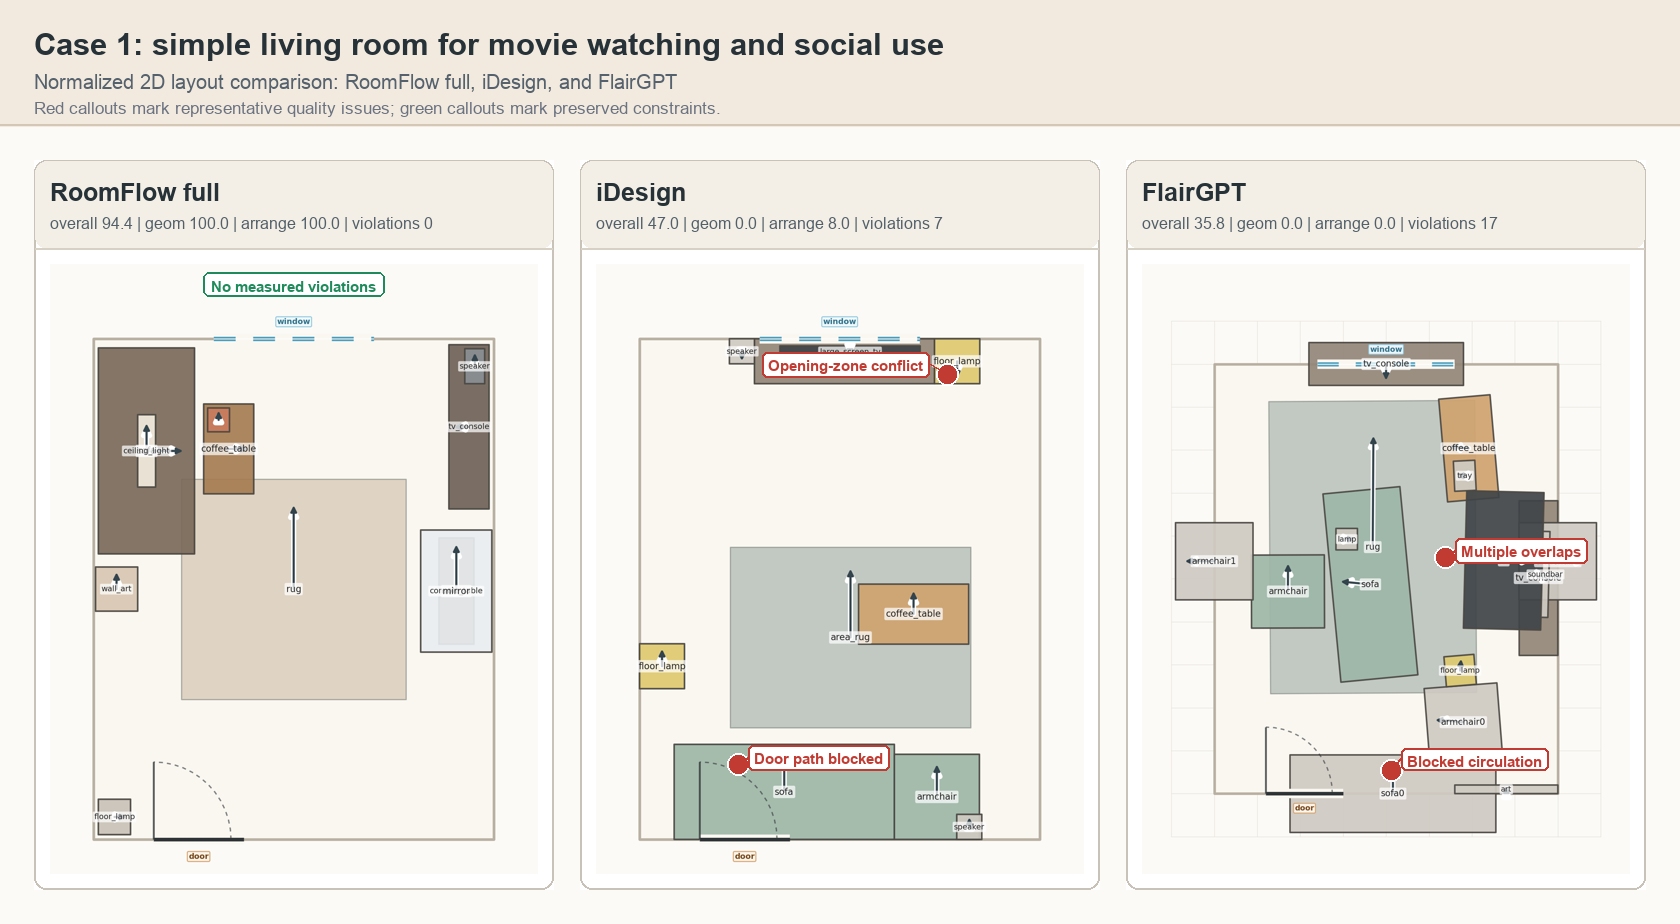
\includegraphics[width=0.96\textwidth]{figures/chapter4/case_comparisons/simple_living_01_comparison.png}
\caption{Simple living room case: 2D layout comparison across RoomFlow full, I-Design, and FlairGPT.}
\label{fig:7-1}
\end{figure}

Figure~\ref{fig:7-1} makes the metric meanings visible in this simple living room. I-Design reaches 100.0 on design brief compliance and usable object completeness because it includes the main requested objects and enough blocking furniture remains usable after basic filtering. Its spatial feasibility score is still 0.0 because the layout blocks openings and paths, and its functional arrangement score drops to 8.0 because the room is difficult to use. RoomFlow full has slightly lower design brief compliance because the optional armchair is not included, but it keeps spatial feasibility and functional arrangement quality at 100.0. This is why the overall score favors RoomFlow: a layout should be editable and usable, not only semantically complete.

\subsection{Example 2: L-Shaped Living Room}
This case tests whether each system respects a non-usable notch while still keeping a circulation path from the entry.

\begingroup
\footnotesize
\begin{verbatim}
Input:
room=living_room
shape=L-shape 5.2m x 4.8m with a 1.6m x 1.8m notch
openings=door on left wall near lower corner; window on top wall
prompt_focus=main seating faces media, entry circulation,
             coffee table, rug, reading chair if possible

Normalized outputs:
RoomFlow: objects=[sofa, tv_console, coffee_table, armchair, rug]
          score=(overall 100.0, spatial 100.0, brief 100.0,
                 functional 100.0, usable 100.0), violations=0
I-Design: objects=[sectional_sofa, media_console, coffee_table]
          score=(overall 39.3, spatial 0.0, brief 77.8,
                 functional 14.0, usable 82.0), violations=7
FlairGPT: objects=[sofa, shoe_bench, tv_console, coffee_table]
          score=(overall 42.2, spatial 0.0, brief 88.9,
                 functional 0.0, usable 100.0), violations=12
\end{verbatim}
\endgroup

\begin{figure}[!htbp]
\centering
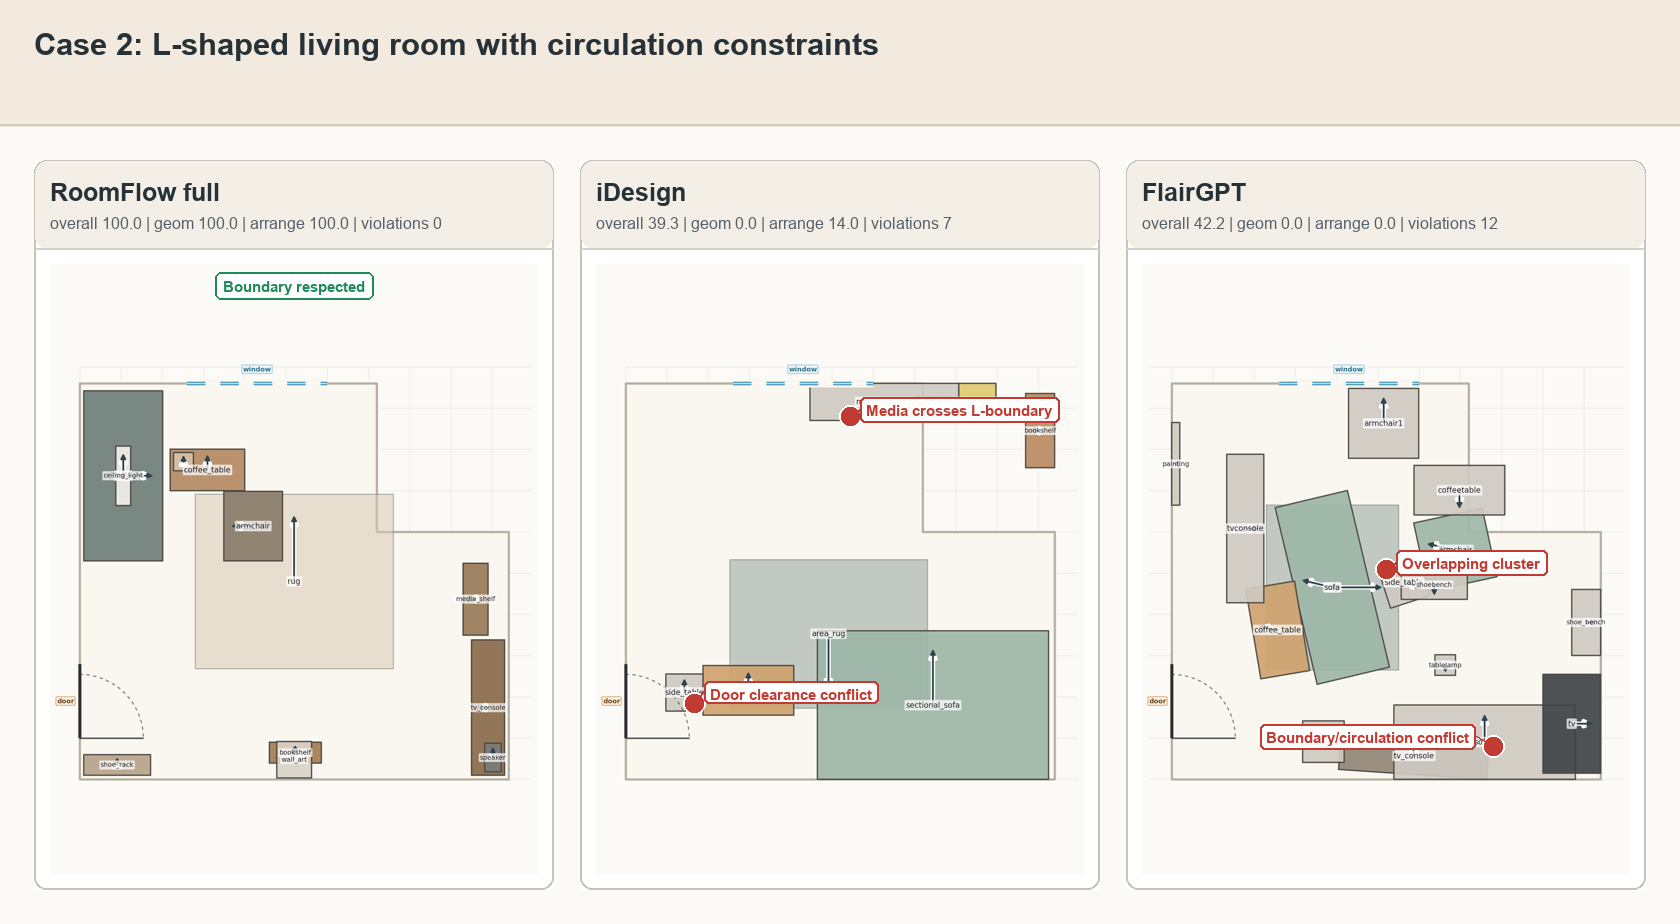
\includegraphics[width=0.96\textwidth]{figures/chapter4/case_comparisons/living_l_shape_comparison.png}
\caption{L-shaped living room case: 2D layout comparison across RoomFlow full, I-Design, and FlairGPT.}
\label{fig:7-2}
\end{figure}

Figure~\ref{fig:7-2} shows why the L-shaped living room is harder: the layout must use the main zone and side wing without crossing the non-rectangular boundary. FlairGPT has a high usable object completeness score because many objects are present and not all are filtered out by count rules, but its spatial feasibility and functional arrangement scores are 0.0 because several objects violate the shape and circulation constraints. RoomFlow full scores 100.0 across all four primary metrics because the same objects are both requested and physically usable. This case shows why usable object completeness must be read together with spatial feasibility.

\subsection{Example 3: Chamfered Bedroom with Openings}
This case combines a clipped corner, required bedroom objects, a door, and a window.

\begingroup
\footnotesize
\begin{verbatim}
Input:
room=bedroom
shape=4.4m x 4.0m with a chamfered upper-right corner
openings=door bottom 0.6-1.5m; window left wall 2.0-3.2m
prompt_focus=bed, wardrobe, compact desk, nightstand,
             curtains, ceiling light

Normalized outputs:
RoomFlow: objects=[bed, wardrobe, desk, nightstand, curtain]
          score=(overall 100.0, spatial 100.0, brief 100.0,
                 functional 100.0, usable 100.0), violations=0
I-Design: objects=[bed, wardrobe, desk, nightstand]
          score=(overall 52.7, spatial 9.1, brief 81.8,
                 functional 38.0, usable 100.0), violations=5
FlairGPT: objects=[bed, wardrobe, compact_desk, nightstand]
          score=(overall 31.9, spatial 0.0, brief 90.9,
                 functional 0.0, usable 46.0), violations=9
\end{verbatim}
\endgroup

\begin{figure}[!htbp]
\centering
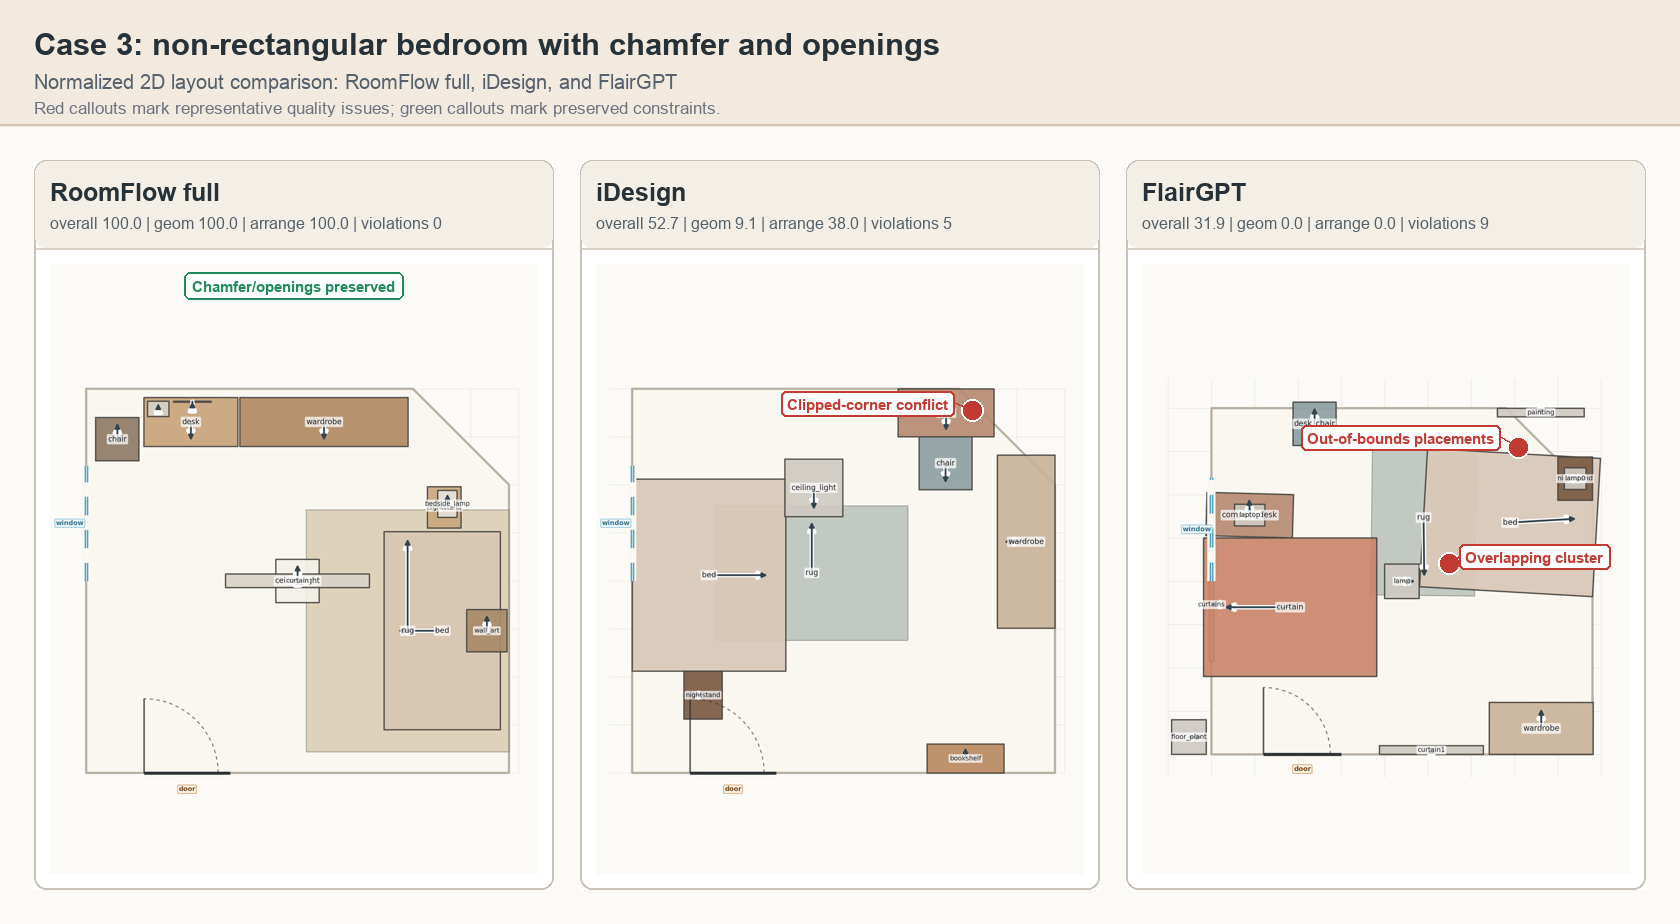
\includegraphics[width=0.96\textwidth]{figures/chapter4/case_comparisons/bedroom_chamfer_comparison.png}
\caption{Chamfered bedroom case: 2D layout comparison across RoomFlow full, I-Design, and FlairGPT.}
\label{fig:7-3}
\end{figure}

Figure~\ref{fig:7-3} illustrates the chamfered bedroom case, which combines non-rectangular geometry with door and window constraints. I-Design and FlairGPT follow several object-name requirements, so their design brief compliance scores are not zero. The spatial feasibility scores show the missing part: some placements become invalid under the clipped room polygon, opening-clearance checks, or overlap checks. I-Design still receives 100.0 on usable object completeness because this metric only checks whether the number of remaining valid blocking objects reaches the case minimum after invalid out-of-bound or overlapping objects are discounted; it does not mean that every requested object is geometrically valid. Its low spatial feasibility and functional arrangement scores capture those geometric failures. RoomFlow full satisfies the same main object requirements while also keeping the blocking objects valid and accessible.

\section{Experiment 1: Comparison with External Baselines}
\label{subsec:eval-layout-external-baselines}

Experiment~1 compares the complete RoomFlow pipeline with two external baselines, I-Design and FlairGPT. The purpose is to evaluate whether RoomFlow can generate more usable editable layouts under the same benchmark cases and scoring protocol. The comparison focuses on four aspects: spatial feasibility, design brief compliance, functional arrangement quality, and usable object completeness.

The three systems are evaluated on the 50 benchmark cases described in Section~\ref{subsec:eval-layout-benchmark-cases}. RoomFlow receives the design brief, explicit room polygon, fixed openings, and furniture inventory. I-Design receives the same case information through a structured adapter, including room geometry and object requirements. FlairGPT receives an equivalent text-based description, where the room shape, openings, required objects, and spatial relations are written as a design brief. Table~\ref{tab:external-compared-systems} summarizes the compared systems and the input form used for each one.

\begingroup
\small
\setlength{\tabcolsep}{4pt}
\renewcommand{\arraystretch}{1.15}
\begin{xltabular}{\textwidth}{|>{\raggedright\arraybackslash}p{0.18\textwidth}|>{\raggedright\arraybackslash}p{0.25\textwidth}|>{\raggedright\arraybackslash}X|}
\caption{Compared systems for Experiment~1.}\label{tab:external-compared-systems}\\
\hline
\textbf{System} & \textbf{Role} & \textbf{Input used in this experiment} \\
\hline
RoomFlow full & Proposed complete pipeline & Design brief, room polygon, fixed openings, and furniture inventory \\
\hline
I-Design & External baseline with structured input & Structured case information, including room geometry and object requirements \\
\hline
FlairGPT & External baseline with text-based input & Textual description of room shape, openings, required objects, and spatial relations \\
\hline
\end{xltabular}
\endgroup

To ensure a fair comparison, all generated outputs are converted into the same normalized layout schema before scoring. This schema records each object's category, footprint, position, and orientation. The same evaluator is then applied to all systems. The following subsections report the results by scenario group: minimal rectangular scenarios, detailed rectangular scenarios, detailed non-rectangular scenarios, and overall paired comparison.

\subsection{Minimal Rectangular Scenarios}

The minimal rectangular scenarios use rectangular rooms and short design briefs. They are included as sanity cases before detailed object relations and irregular geometry are introduced. The design brief compliance check in this group is intentionally simpler than in later groups, because these cases mainly test whether a system can produce a basic usable room. Table~\ref{tab:minimal-rectangular-results} reports the comparison for minimal rectangular scenarios, split by whether fixed openings are present.

\begingroup
\footnotesize
\setlength{\tabcolsep}{2pt}
\renewcommand{\arraystretch}{1.25}
\begin{table}[!htbp]
\centering
\caption{External baseline results for minimal rectangular scenarios.}
\label{tab:minimal-rectangular-results}
\begin{tabularx}{0.985\textwidth}{|>{\raggedright\arraybackslash}p{1.9cm}|>{\raggedright\arraybackslash}p{2.1cm}|>{\centering\arraybackslash}p{1.95cm}|*{4}{>{\centering\arraybackslash}X|}}
\hline
\begin{tabular}[c]{@{}l@{}}\textbf{Opening}\\\textbf{condition}\end{tabular} & \textbf{System} & \begin{tabular}[c]{@{}c@{}}\textbf{Overall}\\\(\mu \pm \sigma\)\end{tabular} & \textbf{Spatial} & \textbf{Brief} & \textbf{Function} & \textbf{Usable} \\
\hline
Without & RoomFlow full & 93.3 \(\pm\) 9.4 & \textbf{100.0} & 82.5 & \textbf{100.0} & 88.3 \\
\hline
Without & I-Design & \textbf{99.4} \(\pm\) 2.8 & 98.7 & \textbf{100.0} & 99.1 & \textbf{100.0} \\
\hline
Without & FlairGPT & 61.3 \(\pm\) 25.9 & 37.1 & 80.0 & 53.4 & 83.8 \\
\hline
With & RoomFlow full & \textbf{87.9} \(\pm\) 9.6 & \textbf{97.6} & 70.0 & \textbf{98.0} & 82.9 \\
\hline
With & I-Design & 73.7 \(\pm\) 11.5 & 46.8 & \textbf{100.0} & 58.8 & \textbf{100.0} \\
\hline
With & FlairGPT & 49.3 \(\pm\) 15.7 & 11.9 & 85.0 & 24.4 & 91.9 \\
\hline
\end{tabularx}
\end{table}
\endgroup

In rooms without openings, I-Design is competitive and slightly exceeds RoomFlow in overall score. I-Design reaches 99.4, while RoomFlow reaches 93.3. Both systems already have near-perfect spatial feasibility and functional arrangement quality in this easy condition. This result shows that the sanity group does not by itself prove the advantage of the proposed solver. Instead, it verifies that the compared systems can all be inspected on simple inputs.

The comparison changes when a door and a window are added. RoomFlow keeps high spatial feasibility and functional arrangement quality, reaching 97.6 and 98.0. I-Design drops to 46.8 in spatial feasibility and 58.8 in functional arrangement quality, although it still satisfies the simplified design-brief checks. FlairGPT also decreases from 61.3 to 49.3 overall. The main benefit of RoomFlow in this group is therefore not about naming objects correctly, but keeping the generated objects usable around fixed openings.

\subsection{Detailed Rectangular Scenarios}

The detailed rectangular scenarios keep the room shape simple but use richer design briefs with required furniture and functional relations. Table~\ref{tab:detailed-rectangular-results} reports the comparison for this group, split by whether fixed openings are present.

\begingroup
\footnotesize
\setlength{\tabcolsep}{2pt}
\renewcommand{\arraystretch}{1.25}
\begin{table}[!htbp]
\centering
\caption{External baseline results for detailed rectangular scenarios.}
\label{tab:detailed-rectangular-results}
\begin{tabularx}{0.985\textwidth}{|>{\raggedright\arraybackslash}p{1.9cm}|>{\raggedright\arraybackslash}p{2.1cm}|>{\centering\arraybackslash}p{1.95cm}|*{4}{>{\centering\arraybackslash}X|}}
\hline
\begin{tabular}[c]{@{}l@{}}\textbf{Opening}\\\textbf{condition}\end{tabular} & \textbf{System} & \begin{tabular}[c]{@{}c@{}}\textbf{Overall}\\\(\mu \pm \sigma\)\end{tabular} & \textbf{Spatial} & \textbf{Brief} & \textbf{Function} & \textbf{Usable} \\
\hline
Without & RoomFlow full & \textbf{100.0} \(\pm\) 0.0 & \textbf{100.0} & \textbf{100.0} & \textbf{100.0} & \textbf{100.0} \\
\hline
Without & I-Design & 96.7 \(\pm\) 5.5 & 96.0 & 95.3 & 97.3 & 99.0 \\
\hline
Without & FlairGPT & 22.6 \(\pm\) 14.4 & 0.0 & 51.6 & 0.2 & 48.0 \\
\hline
With & RoomFlow full & \textbf{92.3} \(\pm\) 22.0 & \textbf{91.4} & 91.9 & \textbf{92.0} & 94.5 \\
\hline
With & I-Design & 72.1 \(\pm\) 10.2 & 48.0 & \textbf{92.6} & 59.0 & \textbf{99.0} \\
\hline
With & FlairGPT & 21.9 \(\pm\) 15.8 & 0.0 & 49.4 & 0.0 & 47.5 \\
\hline
\end{tabularx}
\end{table}
\endgroup

Without openings, RoomFlow and I-Design both perform well. RoomFlow reaches 100.0 overall, while I-Design reaches 96.7. This shows that common rectangular rooms are manageable for both workflows when there are no strong door or window constraints.

With openings, the difference becomes clearer. RoomFlow reaches 92.3 overall, while I-Design drops to 72.1. Their design brief compliance scores remain close, but RoomFlow is much stronger in spatial feasibility and functional arrangement quality. This shows that including the requested objects is not enough; the objects must also remain usable around doors, windows, and circulation space. FlairGPT stays near 22 overall in both conditions because its placements are usually not spatially feasible even when some requested objects are present.

\subsection{Detailed Non-Rectangular Scenarios}

The non-rectangular scenarios contain L-shaped, chamfered, side-recess, and bay-like rooms. This group is more difficult because the system must satisfy the same design brief while respecting irregular room boundaries. Table~\ref{tab:nonrectangular-results} reports the comparison for this group, split by whether fixed openings are present.

\begingroup
\footnotesize
\setlength{\tabcolsep}{2pt}
\renewcommand{\arraystretch}{1.25}
\begin{table}[!htbp]
\centering
\caption{External baseline results for non-rectangular scenarios.}
\label{tab:nonrectangular-results}
\begin{tabularx}{0.985\textwidth}{|>{\raggedright\arraybackslash}p{1.9cm}|>{\raggedright\arraybackslash}p{2.1cm}|>{\centering\arraybackslash}p{1.95cm}|*{4}{>{\centering\arraybackslash}X|}}
\hline
\begin{tabular}[c]{@{}l@{}}\textbf{Opening}\\\textbf{condition}\end{tabular} & \textbf{System} & \begin{tabular}[c]{@{}c@{}}\textbf{Overall}\\\(\mu \pm \sigma\)\end{tabular} & \textbf{Spatial} & \textbf{Brief} & \textbf{Function} & \textbf{Usable} \\
\hline
Without & RoomFlow full & \textbf{100.0} \(\pm\) 0.0 & \textbf{100.0} & \textbf{100.0} & \textbf{100.0} & \textbf{100.0} \\
\hline
Without & I-Design & 82.6 \(\pm\) 6.3 & 59.3 & 96.9 & 82.5 & \textbf{100.0} \\
\hline
Without & FlairGPT & 0.0 \(\pm\) 0.0 & 0.0 & 0.0 & 0.0 & 0.0 \\
\hline
With & RoomFlow full & \textbf{99.7} \(\pm\) 0.9 & \textbf{100.0} & \textbf{98.7} & \textbf{100.0} & \textbf{100.0} \\
\hline
With & I-Design & 46.9 \(\pm\) 26.8 & 17.6 & 68.4 & 35.9 & 77.9 \\
\hline
With & FlairGPT & 31.7 \(\pm\) 9.8 & 0.0 & 69.9 & 0.0 & 71.2 \\
\hline
\end{tabularx}
\end{table}
\endgroup

RoomFlow remains stable across both conditions, reaching 100.0 overall without openings and 99.7 with openings. I-Design performs reasonably without openings, reaching 82.6 overall, but drops to 46.9 when irregular geometry is combined with doors and windows. Its spatial feasibility score also drops from 59.3 to 17.6, showing that openings amplify the difficulty of non-rectangular layout generation.

FlairGPT recovers some design brief compliance and usable object completeness in the larger opening branch, but its spatial feasibility and functional arrangement quality remain 0.0. The 0.0 result in the no-opening branch should be interpreted carefully because it comes from execution failures on a small subset. The main conclusion is therefore that RoomFlow remains usable under irregular geometry and fixed openings, while the tested baselines are much less reliable in this setting.

\subsection{Overall Paired Comparison}

\begin{figure}[!htbp]
\centering
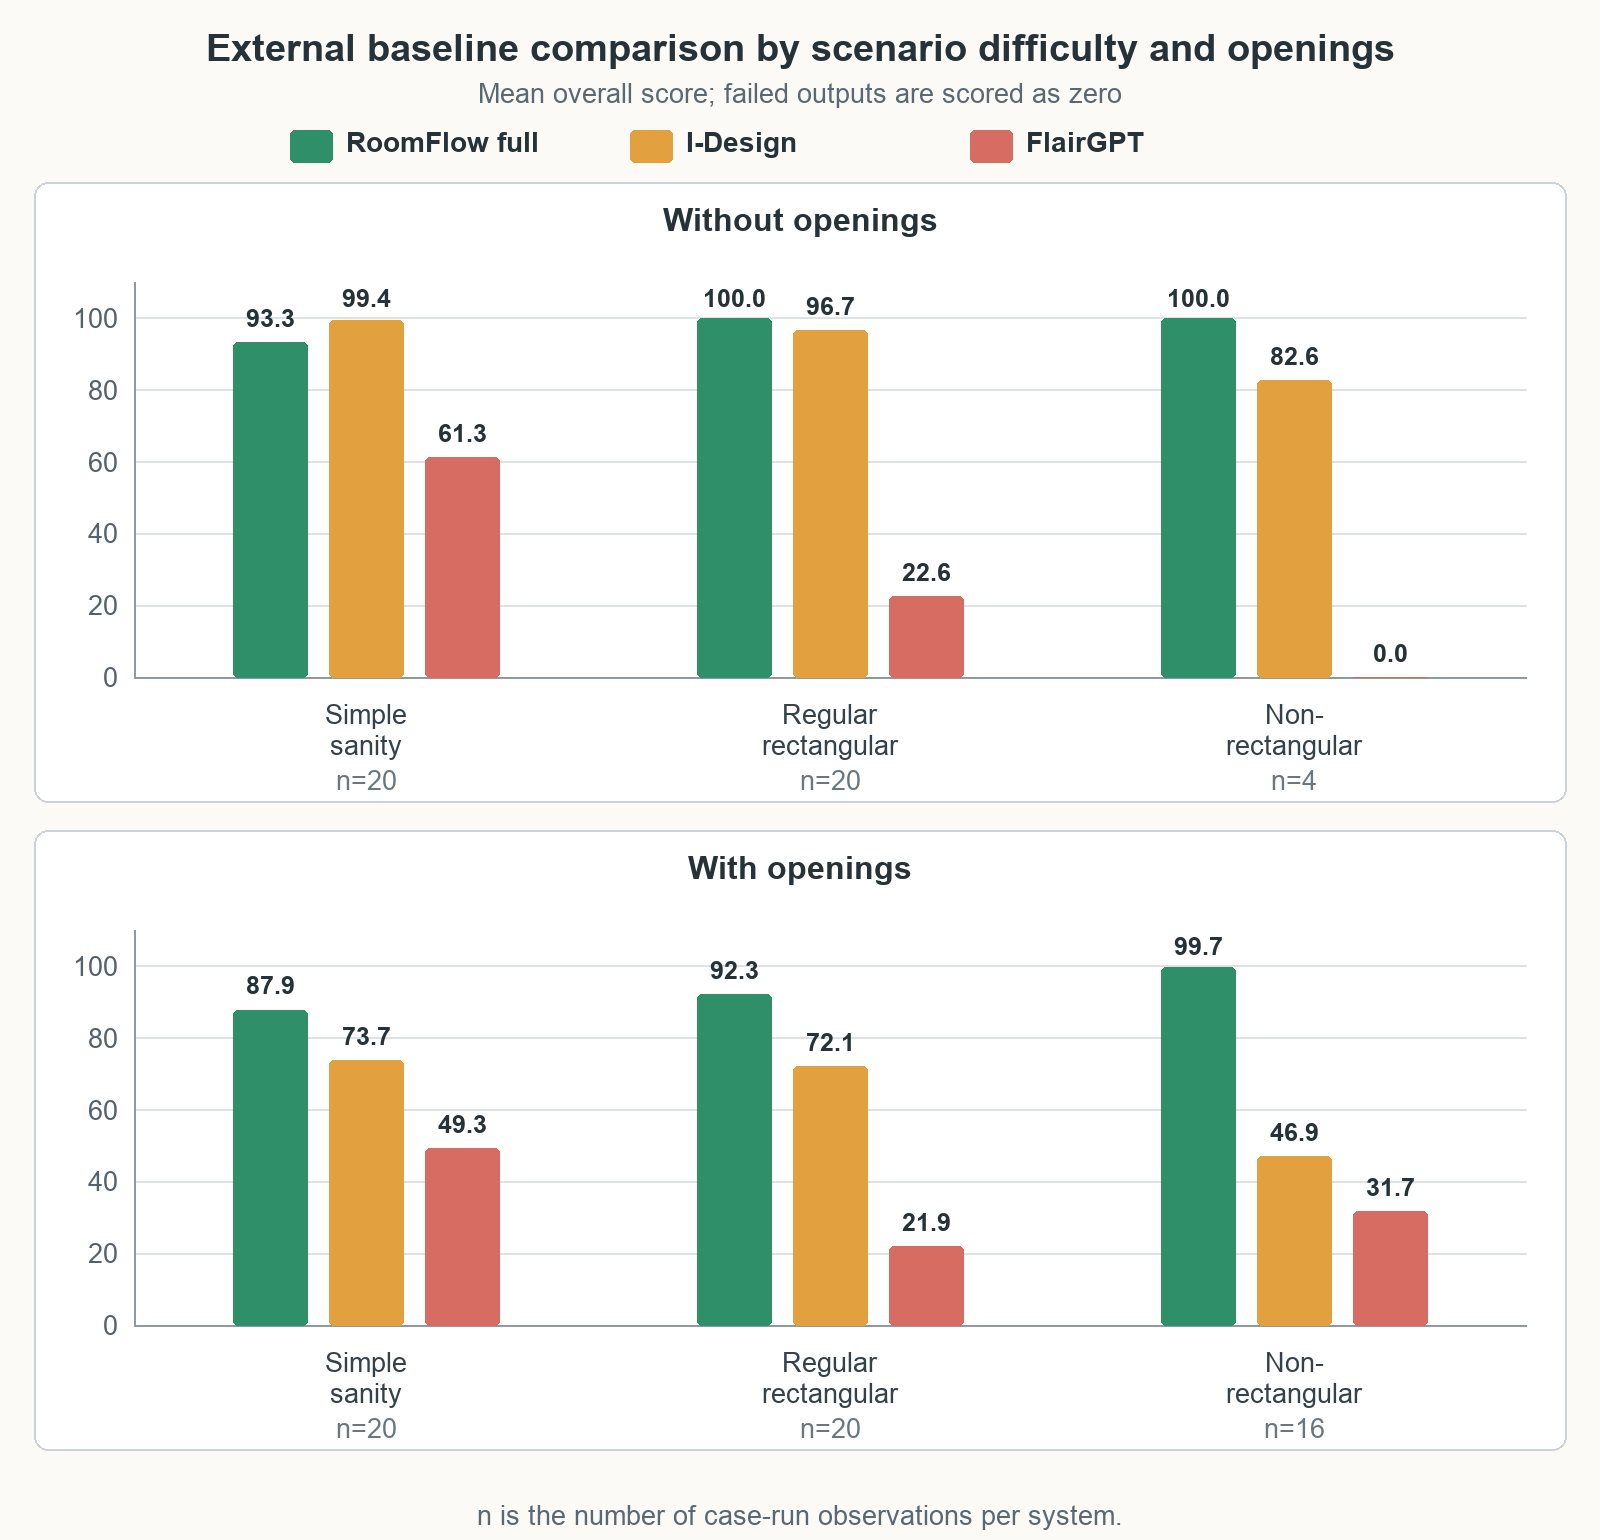
\includegraphics[width=0.98\textwidth]{figures/chapter4/figure_09_grouped_openings.png}
\caption{Overall layout score by scenario group and opening condition.}
\label{fig:7-4}
\end{figure}

Figure~\ref{fig:7-4} summarizes the same pattern across the three scenario groups. In easy rooms without openings, solver-based validation has limited room to improve the result, so I-Design can match or exceed RoomFlow in some cases. The difference becomes clearer when the room contains doors, windows, or non-rectangular boundaries. In these cases, RoomFlow preserves room geometry and functional arrangement more reliably, while the baselines may still include the requested objects but place them in unusable positions.

\begin{figure}[!htbp]
\centering
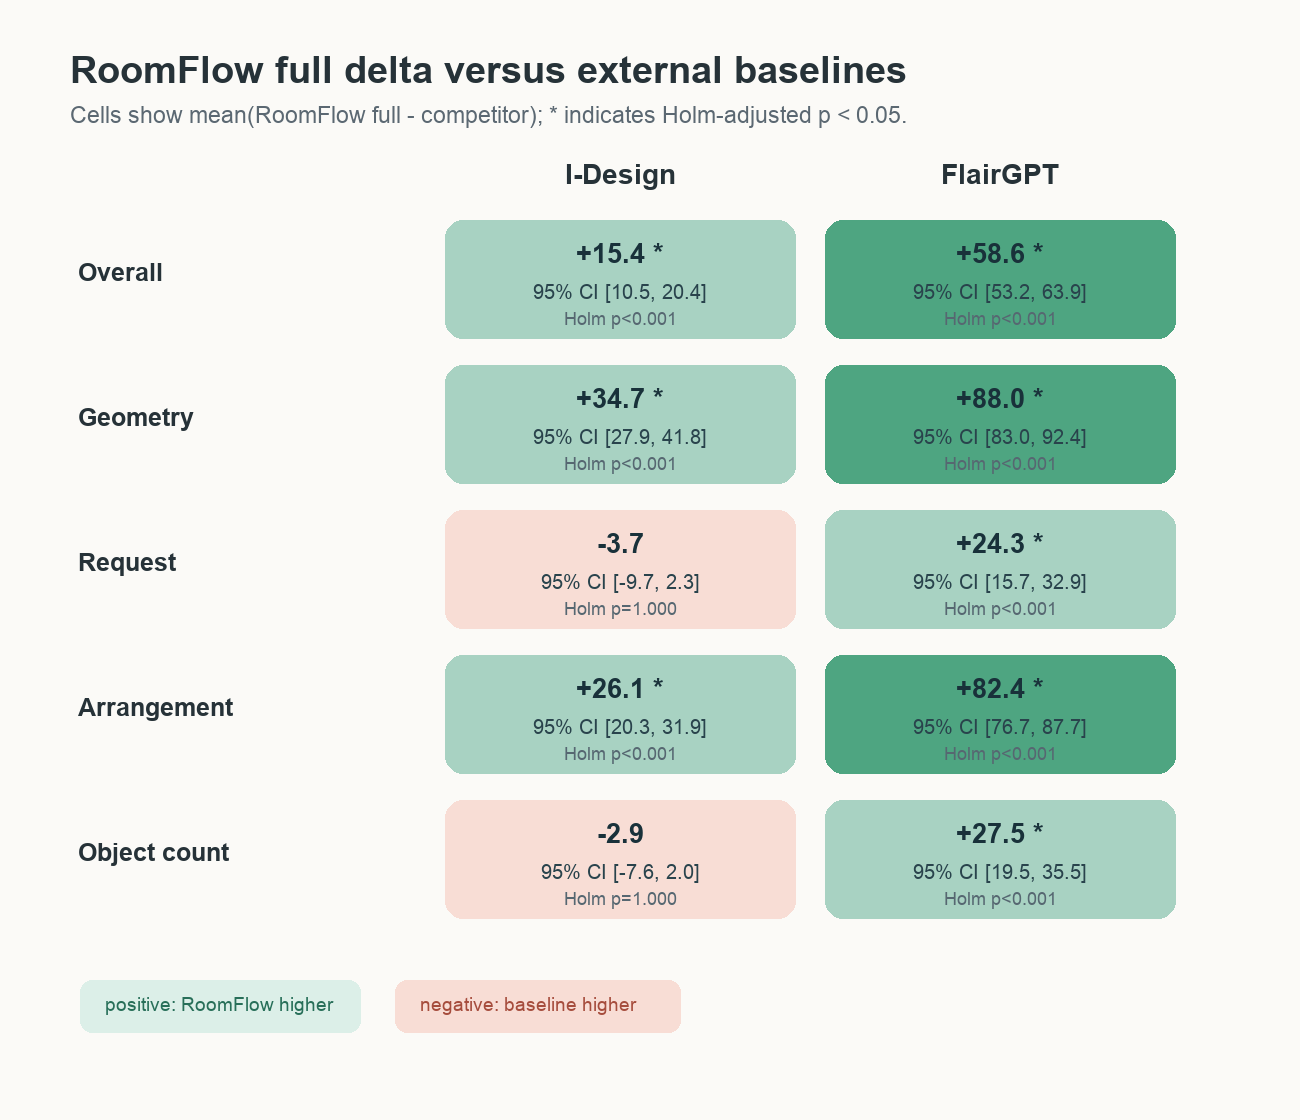
\includegraphics[width=0.92\textwidth]{figures/chapter4/figure_10.png}
\caption{Paired delta of RoomFlow full against I-Design and FlairGPT.}
\label{fig:7-5}
\end{figure}

Figure~\ref{fig:7-5} provides the pooled paired statistics that summarize, rather than replace, the subgroup analysis. Against I-Design, RoomFlow full improves overall score by +15.4 points with a 95\% confidence interval of [10.5, 20.4] and Holm-adjusted p < 0.001. It also improves spatial feasibility by +34.7 and functional arrangement quality by +26.1. Against FlairGPT, all reported deltas are positive and significant, including +58.6 overall, +88.0 spatial feasibility, +82.4 functional arrangement quality, and +27.5 usable object completeness.

\clearpage
\section{Experiment 2: Ablation Study}\label{subsec:eval-layout-ablation}

Experiment~2 evaluates the internal contribution of the main RoomFlow components. Unlike Experiment~1, which compares RoomFlow with external baselines, this experiment compares the complete pipeline with ablated variants of itself. Each ablation removes or weakens one mechanism to show which capability is lost when that component is not used.

All variants receive the same benchmark input and are evaluated with the same scoring protocol. The comparison uses the four primary metrics: spatial feasibility, design brief compliance, functional arrangement quality, and usable object completeness. A separate robustness holdout is also used to examine style-material consistency, gallery diversity, reliability, and lower-tail failures across repeated runs.

The ablations are grouped into semantic-planning, geometric-solver, and post-processing variants. Semantic-planning ablations test the role of object requirements, priorities, relations, and style or material policy. Geometric-solver ablations test the role of collision checks, opening constraints, and circulation validation. Post-processing ablations test the role of gallery diversification, stylistic refinement, and final layout selection.

\subsection{Primary-Metric Ablation Comparison}

This subsection focuses on how each ablation affects the four primary layout metrics. The variants are organized according to the component groups introduced in Section~\ref{subsec:eval-layout-ablation}, but the discussion here focuses on their measurable impact on spatial feasibility, design brief compliance, functional arrangement quality, usable object completeness, and overall score.

The variant names in Table~\ref{tab:primary-ablation-results} can be read as controlled ``what-if'' settings. \textit{Full} is the complete RoomFlow pipeline. The first group weakens how the system understands the user brief before solving. \textit{No request} removes the step that explicitly marks objects as required, preferred, optional, or forbidden. \textit{No tier} removes the step that decides object quantities and placement priority. \textit{No semantic} weakens the whole intent-understanding stage, while \textit{Minimal context} gives the solver only basic room and prompt information.

The second group removes later refinement steps after candidate placements have been produced. \textit{No style} removes style-preference planning. \textit{No material} removes material metadata. \textit{No stylist} removes the final enrichment step that attaches style and inventory display information to valid layouts. \textit{No gallery} removes duplicate filtering and final selection of distinct layout variants. Table~\ref{tab:primary-ablation-results} reports the primary-metric results for the selected ablation variants.

\begingroup
\small
\setlength{\tabcolsep}{4pt}
\renewcommand{\arraystretch}{1.15}
\begin{xltabular}{\textwidth}{|>{\raggedright\arraybackslash}X|>{\raggedright\arraybackslash}X|>{\raggedright\arraybackslash}X|>{\raggedright\arraybackslash}X|>{\raggedright\arraybackslash}X|>{\raggedright\arraybackslash}X|}
\caption{Selected ablation results on the four primary metrics.}\label{tab:primary-ablation-results}\\
\hline
\textbf{Variant} & \textbf{Overall} & \textbf{Spatial} & \textbf{Brief} & \textbf{Function} & \textbf{Usable} \\
\hline
Full & 95.3 & \textbf{100.0} & 87.0 & \textbf{100.0} & 92.5 \\
\hline
No style & \textbf{97.4} & \textbf{100.0} & 93.3 & \textbf{100.0} & 95.5 \\
\hline
No gallery & 97.3 & \textbf{100.0} & 93.1 & \textbf{100.0} & 95.4 \\
\hline
No stylist & 97.3 & \textbf{100.0} & 92.8 & \textbf{100.0} & 95.5 \\
\hline
No material & 97.1 & 99.5 & 91.9 & 99.6 & \textbf{97.0} \\
\hline
No request & 95.7 & \textbf{100.0} & 87.5 & \textbf{100.0} & 94.0 \\
\hline
No tier & 95.4 & 95.8 & \textbf{94.4} & 95.8 & 95.4 \\
\hline
No semantic & 85.0 & 95.8 & 67.5 & 95.8 & 77.1 \\
\hline
Minimal context & 77.1 & 76.2 & 74.5 & 78.5 & 80.0 \\
\hline
\end{xltabular}
\endgroup

The strongest degradation appears when semantic context is weakened. The full pipeline reaches 95.3 overall, while the no-semantic variant drops to 85.0 and the minimal-context variant drops further to 77.1. These results show that the solver benefits from structured design understanding, including object roles, priorities, relations, and usable object requirements. Without this information, the system can still place some objects, but the final layout becomes less aligned with the intended room design.

Some post-processing ablations obtain slightly higher scores on the four primary metrics. For example, the no-style, no-gallery, and no-stylist variants reach around 97 overall in this primary-metric view. This does not mean that the removed components are unnecessary. The four primary metrics mainly reward immediate spatial feasibility, design brief compliance, functional arrangement quality, and usable object completeness. They do not fully measure style-material consistency, gallery diversity, repeated-run reliability, or worst-case behavior.

The primary-metric comparison therefore shows two points. First, semantic planning has a direct effect on layout quality. Second, some post-processing components mainly affect robustness and final variant quality rather than the immediate primary layout score. For this reason, the next subsection evaluates the same system family on a separate robustness holdout.

\subsection{Extended Robustness Holdout}

The extended robustness holdout evaluates behavior that is not fully captured by the four primary layout metrics. It uses the 10-case holdout introduced in Section~\ref{subsec:eval-layout-benchmark-cases}, where the cases include richer style, material, palette, and gallery-diversity requirements. This evaluation is used only for the ablation experiment because these targets mainly test robustness and final variant quality rather than immediate spatial feasibility. Table~\ref{tab:robustness-holdout-results} reports the selected robustness holdout metrics for the full pipeline and major ablated variants.

\begingroup
\footnotesize
\setlength{\tabcolsep}{3pt}
\renewcommand{\arraystretch}{1.15}
\begin{xltabular}{\textwidth}{|>{\raggedright\arraybackslash}p{2.25cm}|>{\raggedright\arraybackslash}p{2.25cm}|>{\raggedright\arraybackslash}p{2.35cm}|>{\raggedright\arraybackslash}p{1.85cm}|>{\raggedright\arraybackslash}p{2.35cm}|>{\raggedright\arraybackslash}X|}
\caption{Selected robustness holdout metrics for full and major ablated variants.}\label{tab:robustness-holdout-results}\\
\hline
\textbf{Variant} & \begin{tabular}[c]{@{}l@{}}\textbf{Robustness}\\\textbf{summary}\end{tabular} & \begin{tabular}[c]{@{}l@{}}\textbf{Worst-case}\\\textbf{robustness}\end{tabular} & \textbf{Canonical} & \begin{tabular}[c]{@{}l@{}}\textbf{Style and}\\\textbf{material}\end{tabular} & \begin{tabular}[c]{@{}l@{}}\textbf{Gallery}\\\textbf{diversity}\end{tabular} \\
\hline
Full & \textbf{95.0} & \textbf{90.4} & \textbf{97.8} & \textbf{84.6} & \textbf{100.0} \\
\hline
No stylist & 88.3 & 7.4 & 89.6 & 82.3 & 91.7 \\
\hline
No request & 87.8 & 8.1 & 90.6 & 78.3 & 91.7 \\
\hline
No tier & 87.6 & 7.4 & 89.5 & 79.8 & 91.7 \\
\hline
No gallery & 81.4 & 7.4 & 82.0 & 78.1 & 83.3 \\
\hline
No style & 81.2 & 7.4 & 82.1 & 77.2 & 83.3 \\
\hline
No material & 81.1 & 7.4 & 82.4 & 78.1 & 80.6 \\
\hline
\end{xltabular}
\endgroup

The full pipeline performs best on the robustness holdout, reaching 95.0 in robustness summary score, 90.4 in worst-case robustness score, 97.8 in canonical quality, 84.6 in style-material consistency, and 100.0 in gallery diversity. These results show that the complete pipeline is not only strong on average, but also more robust across repeated and style-sensitive cases.

The ablated variants are much weaker in lower-tail behavior. For example, no-stylist, no-request, no-tier, no-gallery, no-style, and no-material variants all fall to around 7--8 in worst-case score, even though some of them looked competitive on the four primary metrics. This confirms that the primary scores alone are not sufficient to judge robustness.

The robustness holdout explains why some post-processing or style-related components should still be kept. Removing style, material, gallery selection, or final styling may not immediately damage containment or object counts, but it reduces robust variant quality, style-material consistency, and gallery diversity. Therefore, the ablation study supports keeping the complete RoomFlow pipeline: semantic planning improves layout quality, while post-processing and style-related modules improve robustness and user-facing variant quality.

\section{Discussion}\label{subsec:eval-layout-discussion}

The layout evaluation supports three conclusions. First, RoomFlow full is stronger than the external baselines on overall layout quality, mainly because it improves spatial feasibility and functional arrangement quality. Second, ablation results show that semantic planning, solver validation, and output selection each contribute different types of robustness. Third, the advantage becomes clearer in difficult rooms, where non-rectangular boundaries and openings expose the limitations of direct or weakly constrained layout generation.

\section{Threats to Validity}\label{sec:eval-layout-threats}

Implementation differences may affect the external comparison because I-Design and FlairGPT prompts and outputs must be converted to the common benchmark schema. The adapters preserve recoverable object categories, footprints, positions, and orientations, and all systems are scored by the same scripts, but conversion quality may still influence the result. The dataset also focuses on controlled living-room and bedroom cases rather than the full diversity of real apartments.

The four primary metrics capture important geometric and functional properties, but they cannot fully represent subjective design preference or professional interior-design quality. Two repeated runs expose some non-deterministic variation but remain a limited sample. The confidence intervals and Holm adjustment reduce overstatement, while the robustness holdout provides additional evidence for the internal comparison; the conclusions still apply to the tested benchmark rather than every possible interior-design task.
